\documentclass{foi}
\usepackage{lipsum}

\vrstaRada{\zavrsni} % \diplomski
\title{Prilagodljiv sustav za smanjenje svjetlosnog zasljepljivanja vozača}

\author{Stjepan Petrović}
\spolStudenta{\musko} % \zensko ili \musko
\mentor{Boris Tomaš}
\spolMentora{\musko} % \zensko ili \musko
\godina{2023}
\mjesec{rujan}
\date{2023}
\status{redoviti}
\indeks{0016150314}
\smjer{Informacijski i poslovni sustavi} % (ili Poslovni sustavi, Ekonomika poduzetništva, Primjena informacijske tehnologije u poslovanju, Informacijsko i programsko inženjerstvo, Baze podataka i baze znanja, Organizacija poslovnih sustava, Informatika u obrazovanju)
\titulaProfesora{Doc. dr. sc.}

\sazetak{Tema rada je izrada prilagodljivog sustava za smanjenje svjetlosnog zasljepljivanja vozača što predstavlja fizički koncept koji čini LCD matrica, dvije web kamere i laptop kao procesna jedinica. Izazov je bio spojiti četiri komponente (komponenta za pozicioniranje očiju vozača, komponenta za pozicioniranje zasljepljujućeg svjetla, komponenta za zaštitu od zasljepljujućeg svjetla i komponenta procesne jedinice zajedno sa ostalim hardverom), od kojih svaka ima svoju važnost i način pristupa, u jedan funkcionalan sustav čiji je koncept realiziran u ovome radu i koji odgovara na pitanje: kako preko kamera prepoznati izvor zasljepljujućeg svjetla i zaštiti oči vozača na način da se preko LCD matrice spriječi prolazak zasljepljujućeg svjetla do očiju vozača. Kako bi se izradio odgovarajući sustav korištena je biblioteka OpenCV (engl. \emph{Open Source Computer Vision Library}) koja je kao projekt pokrenuta od strane Intel korporacije, a pruža softver za strojno učenje i računalni vid u realnom vremenu i korišten je programski jezik Python. Programski kod i \LaTeX \space dokumentacija je verzionizirana na GitHub repozitoriju, kojem se može pristupiti preko poveznice: \url{https://github.com/StjepanPetrovic/Prilagodljiv-sustav-za-smanjenje-svjetlosnog-zasljepljivanja-vozaca}}

\kljucneRijeci{računalni vid; OpenCV; vozilo; zasljepljivanje; LCD; Python;}

\begin{document}

\maketitle

\tableofcontents

\pagestyle{plain}
\chapter{Uvod}

Ovim završnim radom obrađeni su teorijski koncepti na kojima se temelji rad, istražena je literatura, opisan je tijek izrade i konačan rezultat izrade \textbf{prilagodljivog sustava za smanjenje svjetlosnog zasljepljivanja vozača} te je provedeno testiranje sustava.

Programski kod i \LaTeX \space dokumentacija je verzionizirana na GitHub repozitoriju, kojem se može pristupiti preko poveznice: \href{https://github.com/StjepanPetrovic/Prilagodljiv-sustav-za-smanjenje-svjetlosnog-zasljepljivanja-vozaca}{https://github.com/StjepanPetrovic/Prilagodljiv-sustav-za-smanjenje-svjetlosnog-zasljepljivanja-vozaca}.

U nastavku rada za izraz „prilagodljiv sustav za smanjenje svjetlosnog zasljepljivanja vozača koristit će se skraćena inačica „\textbf{sustav protiv zasljepljivanja}“.

\section{Definicija problema}

 Bilo je potrebno napraviti sustav koji u realnom vremenu prepoznaje izvor zasljepljujućeg svjetla te reagira na način da polarizira određeni dio reaktivne komponente (LCD matrice) koja bi se nalazila na vjetrobranskom staklu vozila te na taj način smanji jačinu zasljepljujućeg svjetla ispred vozača u vozilu.

 Na slici \ref{fig:prikaz_sustava_1} može se vidjeti da takav sustav treba imati ulazne uređaje pomoću kojih će vidjeti što se događa u okolini vozača. Za ulazne uređaje su uzete dvije web kamere čiji je sadržaj onoga što vide predstavljen kao narančasti i zeleni okvir na slici \ref{fig:prikaz_sustava_1}, a taj sadržaj će obrađivati istrenirani modeli za računalni vid iz biblioteke OpenCV te će tako procesna jedinica znati gdje se nalaze oči vozača i izvor svjetla koji su predstavljeni kao crveni krugovi odnosno baze valjka na narančastom i zelenom okviru na slici \ref{fig:prikaz_sustava_1}. Kada procesna jedinica to zna, potrebno je pomoću algoritma izračunati koji točno dio LCD matrice treba polarizirati/zatamniti, a taj dio koji treba polarizirati je prikazan na slici \ref{fig:prikaz_sustava_1} kao crveni krug na crnom okviru odnosno intersekcija žutog plašta valjka, koji predstavlja svjetlost, sa crnim okvirom koji predstavlja reaktivnu komponentu (LCD matricu). Interaktivnom grafu sa slike \ref{fig:prikaz_sustava_1} može se pristupiti preko linka: \url{https://www.geogebra.org/m/hvzfyjfz}.


\begin{figure}[h!]
    \centering
    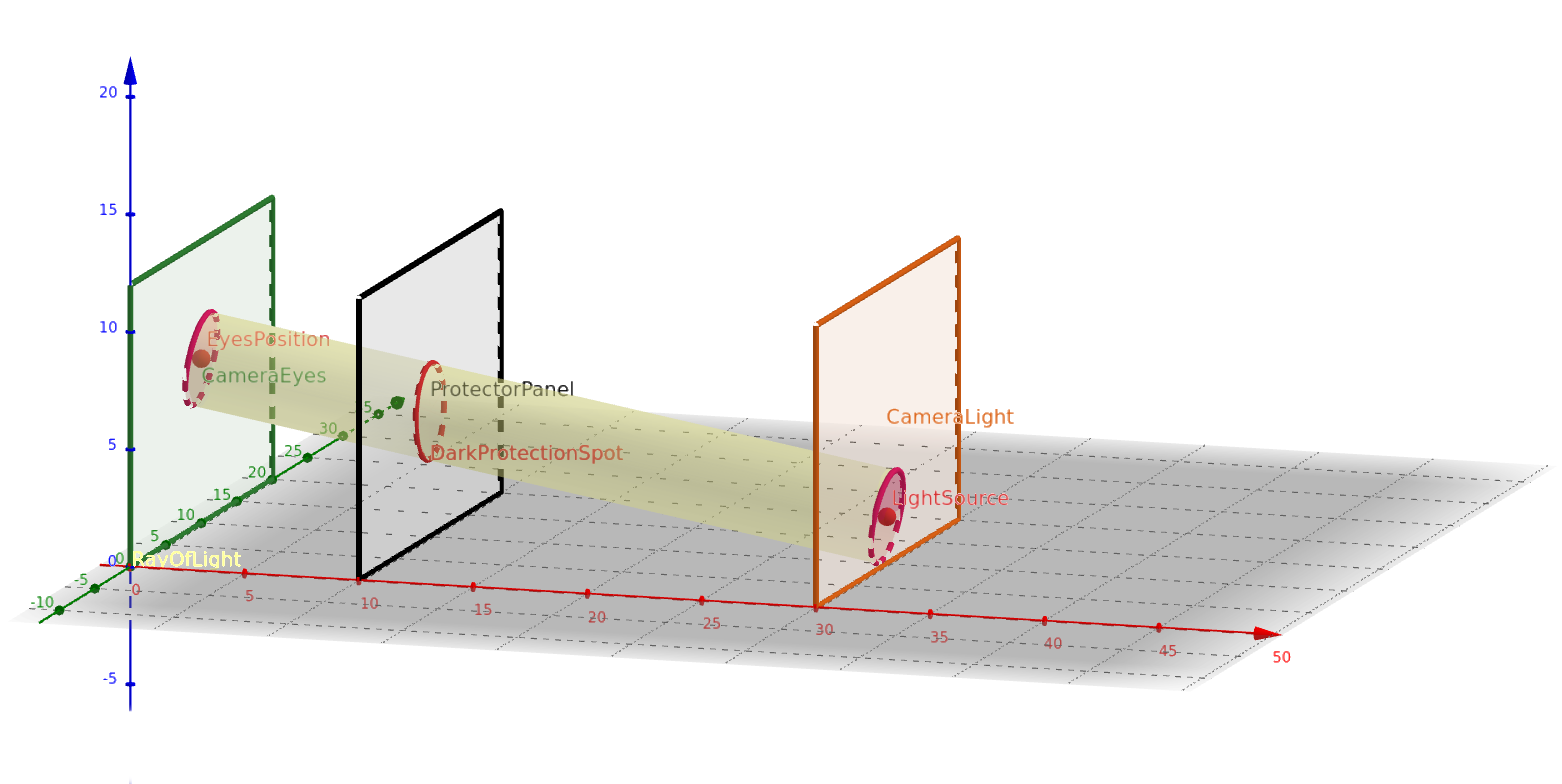
\includegraphics[width=0.75\textwidth]{slike/graf_uvod}
    \captionsetup{font={small}}
    \caption{Pojednostavljen prikaz sustava u trodimenzionalnom koordinatnom sustavu [autorski rad]}
    \label{fig:prikaz_sustava_1}
\end{figure}

Razlog zbog čega je uzeta LCD matrica kao reaktivna komponenta koja će sprječavati zasljepljujuće svjetlo da dođe do očiju vozača je taj što može biti prozirna i moguće je gledati kroz nju, zbog čega neće smetati na vjetrobranskom staklu prilikom vožnje, a lako ju je moguće napraviti neprozirnom na način da se zaslon polarizira odnosno da se pikseli postave na crnu boju.

\begin{flushleft}Sustav protiv zasljepljivanja se sastoji od četiri komponente koje su u radu obrađena:\end{flushleft}
\begin{itemize}[noitemsep]
    \item Procesna jedinica (laptop) i hardver (web kamere i LCD matrica),
    \item Komponenta za prepoznavanje i pozicioniranje izvora svjetla,
    \item Komponenta za prepoznavanje i pozicioniranje očiju vozača,
    \item Komponenta za polarizaciju LCD matrice kao reaktivne komponente.
\end{itemize}

Uz dodatna ulaganja i razvoj, ovaj fizički koncept može postati vrlo popularan i koristan proizvod svakom vozaču u vozilu jer će pružiti zaštitu u noćnoj vožnji od zasljepljujuće svjetlosti, koja usmjerena u oči vozača za vrlo kratak trenutak može ugroziti vozača. Najčešće su izvor te svjetlosti duga svjetla na vozilu vozača koji zbog neopreznosti ne isključi duga svjetla u trenutku kada dolazi ususret drugom vozilu čiji će vozač zbog toga biti svjetlosno zaslijepljen te na trenutak neće moći vidjeti kuda vozi što može loše utjecati na vozača. Zato je bilo potrebno napraviti sustav koji će:
\begin{itemize}[noitemsep]
    \item prepoznati i pozicionirati izvor svjetla te oči vozača koristeći kamere,
    \item kalibrirati komponente i uspješno ih povezati u jedan cjelovit funkcionalan sustav.
\end{itemize}

\section{Motivacija za rad}

Motivacija za odabir ove teme mi je bila misao da ću se okušati u stvaranju sustava protiv zasljepljivanja za kojeg i u modernoj automobilskoj industriji još ne postoji izrađeno rješenje koje je optimalno za korištenje u realnim uvjetima – zbog čega sam gore i rekao da bi uz daljnja ulaganja i razvoj,  fizički koncept koji je izrađen u svrhu ovog završnog rada mogao biti popularan. Postoji velik broj raspisanih patenata od strane najkonkurentnijih svjetskih proizvođača što ostavlja dojam da će skorija budućnost biti jako dinamična utrka za osvajanje tržišta proizvodom koji će, osim borbe sa svjetlosnim zasljepljenjem, donijeti i dodatne mogućnosti kao što je uvođenje proširene stvarnosti (engl. \emph{Augmented Reality - AR}) na vjetrobransko staklo.

Velik je broj nesreća prouzrokovan svjetlosnim zasljepljenjem vozača, a još veći je broj vozila koji se svakim danom povećava na prometnicama širom svijeta, stoga moderna automobilska industrija sve više pokušava proizvesti automobile koji će imati ugrađen takav sustav za zaštitu vozača – što donosi velik značaj ovoj temi te poticaj za daljnje istraživanje i razvoj proizvoda koji će spriječiti povećanje broja prometnih nesreća prouzrokovanih svjetlosnim zasljepljenjem vozača.

\section{Metode i tehnike rada}

U ovom poglavlju treba opisati koje će metode i tehnike biti korištene pri razradi teme, kako su provedene istraživačke aktivnosti, koji su programski alati ili aplikacije korišteni.

\chapter{Pregled literature}

\chapter{Izrada sustava}

\chapter{Testiranje sustava}

\chapter{Zaključak}

Ovdje treba sažeto rezimirati najvažnije rezultate razrade teme rada. Potrebno je sažeto opisati što je predmet rada, koje su metode, tehnike, programski alati ili aplikacije korištene u razradi rada te koje su pretpostavke dokazane, a koje opovrgnute. Sadržajno, ono što se u uvodu rada najavljuje i kasnije je obuhvaćeno u samom radu, moralo bi biti opisano u zaključnom dijelu kroz rezultate rada.

\printbibliography[title=Popis literature]
\addcontentsline{toc}{chapter}{Popis literature}

\listoffigures
\addcontentsline{toc}{chapter}{Popis slika}
 
\listoftables
\addcontentsline{toc}{chapter}{Popis popis tablica}

\end{document}
